\documentclass{beamer}
\usepackage[utf8]{inputenc}
\usepackage{graphicx}
\usepackage{xcolor}
\usepackage{listings}
\usepackage{tikz}

\usetikzlibrary{fit}

\lstdefinelanguage{Tilscript}{
  comment=[l]{--},
  commentstyle={\color{gray}\ttfamily},
  morestring=[b]",
  keywords={Defn, Import, TypeDef, Struct},
  keywordstyle={\color{blue}\ttfamily},
  ndkeywords={Int, Real, Time, World, List, Tuple, If, Progn, MkTuple, Cond,
    ListOf, Bool, Construction, Any1, Any2, Any3, Any4, Any5, Any6, Any7, Any8,
    Any9},
  sensitive=true,
}

\lstset{language=Tilscript}

\title{Implementation of the TIL-Script Language}
\author{Filip Peterek}
\institute{VSB -- Technical University of Ostrava}
\date{May 2023}

\begin{document}

\frame{\titlepage}

\section{Project Goals}

\begin{frame}
    \frametitle{Project Goals}
    \begin{itemize}
        \item Define the TIL-Script programming language
            \begin{itemize}
                \item Build upon the current grammar
                \item Define the semantics of the language
            \end{itemize}
        \item Create a working TIL-Script interpreter
        \item Document the language properly
    \end{itemize}
\end{frame}

\section{Theoretical Background}

\begin{frame}
    \frametitle{Transparent Intensional Logic}
    \begin{itemize}
        \item Logical analysis of natural language
        \item Based on typed Lambda calculi
        \item Rigorously defined type hierarchy
        \item Procedural and hyperintensional
            \begin{itemize}
                \item Constructions can mention other constructions
            \end{itemize}
        \item Sentence meaning is carried by a procedure
            \begin{itemize}
                \item We mostly care for the procedure itself, seldom do we care for the value
                it produces
            \end{itemize}
    \end{itemize}
\end{frame}

\section{TIL-Script}

\begin{frame}
    \frametitle{TIL-Script}
    \begin{itemize}
        \item Grammar closely resembles TIL grammar and conventions
        \item Adds upon TIL to form a useable programming language
            \begin{itemize}
                \item Lists
                \item Tuples
                \item Structures
                \item Strings
            \end{itemize}
        \item Also adds restrictions imposed by computers with finite resources
    \end{itemize}
\end{frame}

\begin{frame}
    \frametitle{Original Features}
    \begin{itemize}
        \item Grammar
        \item All TIL constructions
        \item Type aliases
        \item Lists, Tuples
        \item Semantics not fully defined
    \end{itemize}
\end{frame}

\begin{frame}
    \frametitle{New Features}
    \begin{itemize}
        \item Comments
        \item Imports
        \item Nil value
        \item Distinction between definitions and declarations
        \item String type
        \item Tuples are now heterogenous
        \item Structs (user defined types)
        \item Types as language objects
    \end{itemize}
\end{frame}

\begin{frame}
    \frametitle{Nil Value}
    \begin{itemize}
        \item Used to represent a state when no real value was produced
        \item Internally carries a position in the source code where the value was produced
        \item Also carries the reason as to why a construction was improper
    \end{itemize}
\end{frame}

\begin{frame}
    \frametitle{Declarations And Definitions}
    \begin{itemize}
        \item Declaration only specifies a name and a type
            \begin{itemize}
                \item I.e. if we only know, or only care for, the name
                \item Halting problem -- we may want to refer to it,
                    but we can't solve it
                \item Function Halts/(Bool Program) cannot be implemented
            \end{itemize}
        \item Definition also specifies semantics or value
    \end{itemize}
\end{frame}

\begin{frame}
    \frametitle{Tuples And Lists}
    \begin{itemize}
        \item Originally
            \begin{itemize}
                \item Tuples were homogenous and finite
                \item Lists were homogenous and infinite
            \end{itemize}
        \item Now
            \begin{itemize}
                \item Tuples are heterogenous and fixed in size
                \item Lists are homogenous, size is unlimited
            \end{itemize}
    \end{itemize}
\end{frame}

\begin{frame}
    \frametitle{Structs}
    \begin{itemize}
        \item User defined compound types
        \item Cannot be coerced into other types with same layout
        \item Allows for better use of the TIL-Script type system
            \begin{itemize}
                \item E.g. cartesian vs. polar coordinates
            \end{itemize}
    \end{itemize}
\end{frame}

\begin{frame}[fragile]
\frametitle{Code Example}
    
\begin{lstlisting}[basicstyle=\small]
numbers -> List(Int) := ['ListOf '1 '6 '2 '5 '3 '4].

Defn LessThanFive(num: Int) -> Bool := ['< num '5].

Defn Filter(list: List(Int), pred: (Bool Int))
        -> List(Int) :=
    ['If ['IsEmpty list]
        list
        ['If [pred ['Head list]]
            ['Cons 
                ['Head list] 
                ['Filter ['Tail list] pred]]
            ['Filter ['Tail list] pred]]].

['Println ['Filter numbers 'LessThanFive]].
\end{lstlisting}

\end{frame}

\section{Implementation}

\begin{frame}
    \frametitle{Implementation}
    \begin{itemize}
        \item Kotlin
            \begin{itemize}
                \item Algebraic data types
                \item Null safety
                \item Immutable interfaces for collections
            \end{itemize}
        \item Gradle
        \item Antlr
    \end{itemize}
\end{frame}

\begin{frame}
    \frametitle{Project Structure}

    \begin{figure}
        \centering
        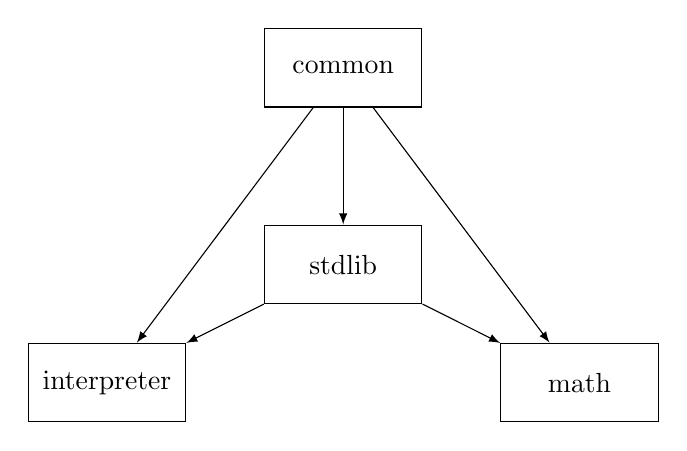
\begin{tikzpicture}
            \node[draw, fit={(0, 0) (2, 1)},                xshift=3cm, inner sep=0pt, label=center:common] (A) {};
            \node[draw, fit={(0, 0) (2, 1)}, yshift=-2.5cm, xshift=3cm, inner sep=0pt, label=center:stdlib] (B) {};

            \node[draw, fit={(0, 0) (2, 1)}, yshift=-4cm,   xshift=6cm, inner sep=0pt, label=center:math] (C) {};
            \node[draw, fit={(0, 0) (2, 1)}, yshift=-4cm,   xshift=0cm, inner sep=0pt, label=center:interpreter] (D) {};

            \draw [-latex]          (A)--(B);
            \draw [-latex]          (A)--(C);
            \draw [-latex]          (A)--(D);
            \draw [-latex]          (B)--(C);
            \draw [-latex]          (B)--(D);
        \end{tikzpicture}
        \caption{Project Structure}
    \end{figure}

\end{frame}

\begin{frame}
    \frametitle{Interpreter Implementation}
    \begin{itemize}
        \item Written in Kotlin
        \item Parser is autogenerated
        \item Functions can be written in TIL-Script or JVM languages
            \begin{itemize}
                \item Allows for access to the entire JVM ecosystem
                \item I.e. database libraries don't have to be implemented from scratch
                \item JDBC can be used
                \item No need to handle syscalls
                \item No need to reimplement math functions
            \end{itemize}
    \end{itemize}
\end{frame}

\begin{frame}
    \frametitle{Interpreter Implementation}
    \begin{itemize}
        \item Object oriented design
            \begin{itemize}
                \item Not the best choice for an interpreter
                \item Simplifies dealing with functions of different implementations
                \item The interpreter can be replaced with a better, drop-in replacement
                \item Limited choice on the JVM
            \end{itemize}
        \item Functional approach where possible
        \item Immutability is preferred
    \end{itemize}
\end{frame}

\section{Current State}

\begin{frame}
    \frametitle{Current State}
    \begin{itemize}
        \item Working prototype
        \item All features work as intended
        \item Lists, tuples, user-defined structures, mutually recursive functions, variables,
            imports, etc.
        \item Type coherency checking
    \end{itemize}
\end{frame}

\begin{frame}
    \frametitle{Limitations}
    \begin{itemize}
        \item Working prototype
        \item No bytecode
            \begin{itemize}
                \item Negative performance implications
                \item Callstack is tied to the JVM callstack
                \item Bytecode conversion must be bijective
            \end{itemize}
        \item No TCO
            \begin{itemize}
                \item Unfortunate, but cannot be done without bytecode
            \end{itemize}
    \end{itemize}
\end{frame}

\begin{frame}
    \frametitle{Possible Improvements}
    \begin{itemize}
        \item REPL
        \item Editor support and an LSP
        \item Compilation to bytecode
    \end{itemize}
\end{frame}

\begin{frame}
    \begin{center}
        \Huge The End
    \end{center}
\end{frame}

\begin{frame}
    \frametitle{Questions}
    \begin{itemize}
        \item What is a degenerate function?
            \begin{itemize}
                \item A function which is undefined on the entirety of its domain
                \item $\lambda x \, . \, x \div 0$
                \item $\lambda x \, . \, log_x 0$
            \end{itemize}
    \end{itemize}
\end{frame}

\end{document}
